\documentclass[UTF8]{article}
%\renewcommand\abstractname{Abstract}
%\renewcommand\contentsname{Content}
%\renewcommand{\thetable}{}
%\usepackage{CTEX}
\usepackage{CJKutf8}
\usepackage{listings}
\usepackage{color}
\usepackage{hyperref}
\hypersetup{colorlinks=true,linkcolor=black}
\definecolor{dkgreen}{rgb}{0,0.6,0}
\definecolor{gray}{rgb}{0.5,0.5,0.5}
\definecolor{mauve}{rgb}{0.58,0,0.82}
\lstset{ %
  language=Octave,                % the language of the code
  basicstyle=\footnotesize,           % the size of the fonts that are used for the code
  numbers=left,                   % where to put the line-numbers
  numberstyle=\tiny\color{gray},  % the style that is used for the line-numbers
  stepnumber=2,                   % the step between two line-numbers. If it's 1, each line
                                  % will be numbered
  numbersep=5pt,                  % how far the line-numbers are from the code
  backgroundcolor=\color{white},      % choose the background color. You must add \usepackage{color}
  showspaces=false,               % show spaces adding particular underscores
  showstringspaces=false,         % underline spaces within strings
  showtabs=false,                 % show tabs within strings adding particular underscores
  frame=single,                   % adds a frame around the code
  rulecolor=\color{black},        % if not set, the frame-color may be changed on line-breaks within not-black text (e.g. commens (green here))
  tabsize=2,                      % sets default tabsize to 2 spaces
  captionpos=b,                   % sets the caption-position to bottom
  breaklines=true,                % sets automatic line breaking
  breakatwhitespace=false,        % sets if automatic breaks should only happen at whitespace
  title=\lstname,                   % show the filename of files included with \lstinputlisting;
                                  % also try caption instead of title
  keywordstyle=\color{blue},          % keyword style
  commentstyle=\color{dkgreen},       % comment style
  stringstyle=\color{mauve},         % string literal style
  escapeinside={\%*}{*)},            % if you want to add LaTeX within your code
  morekeywords={*,...}               % if you want to add more keywords to the set
}
\usepackage{tabularx}
\usepackage{graphicx}
\graphicspath{{fig/}}
\usepackage{enumerate}
\usepackage{geometry}
\geometry{left=1cm,right=1cm,top=2cm,bottom=2cm}
\usepackage{amsmath}
\usepackage{multicol}
\usepackage{indentfirst}
\setlength{\parindent}{2em}
\title{\textbf{How to rationally assess\\
the long-term impact\\
of "takeaways" on the environment}}
\author{}
\date{}
\begin{document}
\begin{CJK}{UTF8}{gkai}
\huge
\begin{center}
2016年美国大学生数学建模竞赛\\
南京理工大学选拔赛\\
\makebox[6em]{}\\
\makebox[6em]{}
\end{center}
\Large
参赛队员详细信息(中文)
\begin{enumerate}
\item	姓名:\underline{吴振宇} \\
学号:\underline{916101630117 }\\
学院:\underline{机械工程学院 }\\
联系电话:\underline{18355528308}\\
\item姓名:\underline{吕俊杰} \\
学号:\underline{9161100Y0124 } \\
学院:\underline{自动化学院} \\
联系电话:\underline{18115023386} \\
\item姓名:\underline{董浩宸} \\
学号:\underline{9161100Y0113} \\
学院:\underline{自动化学院 } \\
联系电话:\underline{18851193695}
\end{enumerate}
\end{CJK}
\newpage
\normalsize
\begin{center}
\begin{tabular}{ccc}
For office use only&Team Control Number&For office use only\\
1.\underline{\makebox[6em]{}}&\underline{\makebox[6em]{320171087}}&1.\underline{\makebox[6em]{}}\\
2.\underline{\makebox[6em]{}}&\makebox[6em]{}&2.\underline{\makebox[6em]{}}\\
3.\underline{\makebox[6em]{}}&Problem Chosen&3.\underline{\makebox[6em]{}}\\
4.\underline{\makebox[6em]{}}&\underline{\makebox[6em]{1}}&4.\underline{\makebox[6em]{}}
\end{tabular}\\
\makebox[6em]{}\\
\makebox[6em]{}\\
\makebox[6em]{}\\
\makebox[6em]{}
\end{center}
\begin{center}
\textbf{2017}\\
\textbf{Mathematical Contest in Modeling (MCM/ICM)
\\Summary Sheet}\\
\end{center}
\maketitle
\begin{abstract}
As the development of online catering industry, more and more problem caused by catering industry has been proposed. However, there is no feasible assessment system related to the long-term impact of "takeaways" on the environment being designed until now. So, we decide to establish a mathematical model to make a estimation about solid waste produced by takeaways from the aspect of classification, proportion etc.\\
\indent The first stage, we establish time series model. We select a typical city which is divided into several districts to collect the data of waste produced in this district. Meanwhile, the proportion of population in respective districts is also be gathered. The solid waste is divided into several kinds, such as paper, metal, plastic, food waste and so on. The proportion of the population of each district to the total population of Shenzhen is regarded as the proportion of all waste in Shenzhen. To use these proportion, we can obtain different weighted average in different classification. Through the number of whole waste, we will forecast the number of different type of solid waste generated in 2017 or further.\\
\indent The second stage, we adopt linear programming model. There are three main treatments employed at present consisting of incineration, landfill and recycling. For each background, we consider the transportation cost, treating cost, health cost, benefit, thus forming several indexes. Then, according to the treatment capacity of Shenzhen waste treatment plant and the quantity of garbage produced in each district, we can determine the linear constraint and objective function based on total cost. In addition, we considered two options, the difference being that the latter implemented garbage sorting first, thus reducing the amount of garbage. Through the corresponding programming software, optimal solution of the minimum total cost will come to be and we consider it to be the best scheme.\\
\indent The third stage, we mainly take advantage of the principal component regression analysis. By selecting four indexes of overtime rate, average staying time, average income and consumption level, the relationship between the production quantity per capita and the characteristics of residents in 2017 was obtained by selecting the first two principal components to ensure that the contribution rate was above 88\%. By correlation coefficient, we can obtain the corresponding relationship between takeaways’ order quantity and the habits of residents, thus set up our evaluation model. The 2 principal components can be interpreted as the principal component of the economic level and the principal component of the quality of life.\\\\
\textbf{Key words:} takeaways\ \  \ \ solid waste\ \  \ \ time series model\ \ \ \  linear programming\ \  \ \ principal component regression analysis
\end{abstract}
\newpage
\tableofcontents

\newpage
\section{Introduction}
\subsection{Background}
An article posted in September 2017, titled "Takeaways Are Destroying Our Next Generation", aroused public attention. According to data released by the take-away platform Are You Hungry and the Industry Research Report from the third-party research company iResearch, it reached the following conclusions, "At least 400 million takeaways are delivered per week in China's streets and alleys, which result in the disposal of at least 400 million one-time boxes and 400 million plastic bags, and 400 million disposable tableware". However, it takes 470 years for a plastic bag to degrade, so plastic bags are very harmful that could ruin our next generation's survival and endanger the planet's future ecology.\\
\indent There are some opposing views according to the research studied by experts related to environment that the environment should be improved if residents could raise their awareness of their duty. Meanwhile, takeaway platform need to reflect their operating strategy.\\
\indent It is urgent for the whole community to construct an assessable criterion to help us realize the impact on the environment caused by solid waste, especially takeaways.
\subsection{Restatement of problem}
Problem 1: In the community where we live, estimate the number of the solid waste caused by takeaways which could be divided into different classification.\\
\indent Problem 2: research and finish quantitative analysis of treatment of various types of solid waste and also propose more optimized and feasible treatment options.\\
\indent Problem 3: Using the data released by some agencies and your first-hand data, quantitatively study the relationship between solid waste caused by takeaways and the characteristic of the residents. On the basis of collecting data, establish a reasonable and rigorous mathematical model to conduct research and propose a research report with quantitative analysis, which should include data sources, reliability, relevant reference materials and so on.
\subsection{Current situation}
At present, takeaways take up a large proportion in catering industry and almost become a necessity in human’s daily life. While, the waste caused by takeaways bring a catastrophic destroy for our environment, especially the plastic, which needs to take hundreds of years to degrade completely. What’s more, regrettably, neither of the perspective which exists lacks a sufficient rational basis, especially the support of quantitative analysis. We believe that our model will work at this situation.
\newpage

\section{Analysis of the problem}
There are three main tasks in this paper and they are:\\
\begin{enumerate}
\item Estimating the number of different type of waste. According to the past information, we can predict the data in the future, thus take actions to protect our environment.\\
\item Confirming the whole cost by utilizing some cost index and propose an optimized and feasible solution. Through this solution, we can provide a sufficient treatment for governments to popularize in wide scope.\\
\item Choosing several cities and formulating some indexes about the characteristic of residents to calculate waste produced by takeaways.
Besides, some necessary information is found on the Internet, so that we can build our own model consisted with the facts.
\end{enumerate}
\newpage

\section{General assumptions}
\noindent Problem 1:\\
\begin{enumerate}
\item For the first problem, we assume that the number of various types of waste is in direct proportion to the population in per district.\\
\item The amount of waste transported is equal to the total amount of waste.\\
\item The number of waste in the city remains steady growth and there is no excessive fluctuation in recent years.
\end{enumerate}
Problem 2:\\
\begin{enumerate}
\item For the second problem, the result derived from the first question is true.\\
\item On the basis of the definition of particle in physics, we assume that the waste is produced at some point intensively and these areas are called "CBD".\\
\item There is no situation that the waste is discarded in the district surveyed and incineration, landfill and recycling are the only three treatments.\\
\item In the policy level, the current implementation of the subsidy policy in classification collection gets the positive response from citizens and all the waste will be classified.\\
\item The whole refuse landfill and waste incineration plant are operating in their scope of processing capacity and the overload operation doesn’t exist.\\
\item All the waste which could recycle can be harnessed again and the product can work off in market price in total.\\
\item The ash which comes from the incineration is ignored and we just consider the health cost caused by its contamination.\\
\item We assume that the discount rate and rate of inflation remain invariable in short time.\\
\item The pollution caused by incineration and landfill is the main reason that residents are afflicted with cancer and subordinate reasons are neglected.\\
\item The more optimized scheme is the minimum total cost.
\end{enumerate}
Problem 3:\\
\begin{enumerate}
\item For the third problem, the takeaways’ order quantity is relative to the overtime rate, average time of staying up late, average revenue and consumer price index.
\end{enumerate}
\newpage
\section{Definitions}
\begin{table}[hpt]
\caption{the definitions of the variables}
\begin{center}
\begin{tabular}{cl}
\hline
Variable&Definition \\
\hline
\(q_{ij}(k)\) &Proportion of \(j\) type of waste in \(i\) district to the total city in \(2015+k\)\\
\hline
\(w_i(k)\)&Proportion of population in \(i\) district to the total city in \(2015+k\)\\
\hline
\(q_j(k)\)&Proportion of \(j\) type of waste to the total waste in \(2015+k\)\\
\hline
\(Q(k)\)&The total number of waste in \(2015+k\)\\
\hline
\(Q_j(k)\)&The total number of \(j\) type of waste in \(2015+k\)\\
\hline
\(a_i\)&The total number of waste in \(i\) district\\
\hline
\(b_j\)&The capacity of the \(j\) waste incinerator or landfill plant\\
\hline
\(d_{ij}\)&The distance between ``CBD'' in \(i\) district and the \(j\) waste treatment plant\\
\hline
\(p\)&Freight of delivering per kilometer per ton of waste\\
\hline
\(c_{ij}\)&Freight of delivering per kilometer per ton of waste in \(i\) district to the \(j\) waste treatment plant\\
\hline
\(q_j\)&The proportion of \(j\) type of recycled waste to total waste\\
\hline
\(m_j\)&Benefit from \(j\) type of per ton of recyclable waste\\
\hline
\(x_{ij}\)&The total number of the waste delivered to the \(j\) plant in \(i\) district\\
\hline
\(P\)&The total cost of garbage disposal\\
\hline
\(P_1\)&The cost of transportation\\
\hline
\(P_2\)&The cost of treatment\\
\hline
\(P_3\)&The cost of health\\
\hline
\(y\)&The amount of waste produced by takeaways per person in 2016\\
\hline
\(x_1\)&Overtime rate in 2016\\
\hline
\(x_2\)&Average time of staying up late in 2016\\
\hline
\(x_3\)&Average revenue in 2016\\
\hline
\(x_4\)&Consumer price index in 2016\\
\hline
\(n_{\textrm{m}}\)&The monthly amount on average orders of the city in 2016\\
\hline
\(n_{\textrm{p}}\)&The population of the city in 2016\\
\hline
\(r\)&The rate of waste produced by takeaways of the city to the average of the whole nation in 2016\\
\hline
\(t_{\textrm{sleep}}\)&The average time of sleep\\
\hline
\(t_{\textrm{wake\ up}}\)&The average time of wake up\\
\hline
CPI&Consumer price index\\
\hline
\(k_l\)&The coefficient of the \(x_l\)\\
\hline
\(k_0\)&The intercept\\
\hline
\(R\)&Correlation coefficient matrix\\
\hline
\(\Lambda\)&Eigenvalue matrix\\
\hline
\(C\)&Contribution matrix\\
\hline
\(V\)&Orthogonal matrix\\
\hline
\(v_l\)&The eigen vector of the order of \(l\)\\
\hline
\(S\)&Score matrix\\
\hline
\(z_1\)&The quality of life of principal component\\
\hline
\(z_2\)&The economic level of principal component\\
\hline
\end{tabular}
\end{center}
\end{table}
\newpage

\section{Model I}
Since we need to estimate the number of solid waste, it is necessary for us to harness the past information and forecast the data in the future. So, we adopt single exponential smoothing to predict the number of various type of waste. Since the data fluctuate within a certain range, single exponential smoothing could predict the data precisely.
\subsection{Collection of the Data}
The following table includes a sample survey of municipal solid waste (MSW) from municipal solid waste (MSW) disposal sites in Shenzhen in 2005. A four-phase survey was conducted in Baoan District in 2006-2007 and a survey on garbage characteristics in Luohu District in 2008. In 2010, the investigation was carried out on Futian District and Luohu District. In 2011, a sampling survey was carried out on the municipal solid waste (including Nanshan incinerator, Yantian incinerator, Xiaping landfill, duck lake landfill, Pinghu incinerator, Tiger pit environment park) in Shenzhen.\footnote{The data comes from reference 1.}
\begin{table}[h]
\caption{}
\begin{center}
\begin{tabular}{ccccp{1cm}cccccc}
\hline
Administrative Region&Year&Kitchen waste&Paper&Rubber and plastic&Fabric&Wood&Dirt&Tile&Glass&Metal\\
\hline
Luohu&2005&57.70\%&9.94\%&10.53\%&3.53\%&7.87\%&4.30\%&1.51\%&3.30\%&1.32\%\\
\hline
Futian&2005&58.96\%&10.35\%&7.88\%&3.35\%&8.43\%&4.48\%&1.26\%&3.81\%&1.48\%\\
\hline
Nanshan&2005&47.29\%&9.80\%&17.20\%&10.80\%&5.60\%&3.53\%&1.28\%&3.10\%&1.40\%\\
\hline
Yantian&2005&50.62\%&8.24\%&13.30\%&7.72\%&6.74\%&7.96\%&1.92\%&2.63\%&0.87\%\\
\hline
Baoan&2005&45.58\%&7.11\%&19.85\%&8.25\%&2.99\%&10.21\%&2.23\%&2.84\%&0.94\%\\
\hline
Longgang&2005&46.82\%&5.19\%&19.53\%&7.84\%&3.89\%&10.68\%&2.53\%&2.61\%&0.91\%\\
\hline
Baoan&2007&37.53\%&12.17\%&19.35\%&9.36\%&2.81\%&13.77\%&2.81\%&1.25\%&0.63\%\\
\hline
Luohu&2008&45.98\%&18.44\%&15.90\%&3.28\%&2.89\%&7.35\%&3.59\%&0.72\%&1.95\%\\
\hline
Luohu&2010&51.99\%&15.31\%&26.44\%&1.03\%&1.29\%&0.00\%&1.42\%&2.19\%&0.13\%\\
\hline
Futian&2010&56.75\%&11.15\%&22.92\%&2.23\%&1.49\%&0.00\%&0.25\%&4.58\%&0.62\%\\
\hline
\end{tabular}
\end{center}
\end{table}\\
\indent The following table is the sampling survey conducted by Shenzhen Environmental Sanitation Administration in 2011 on the various waste proportions of each waste treatment plant ( the area of each waste treatment plant has been marked and its approximate view is regarded as the proportion of various garbage in the area )\footnote{The data comes from reference 1.}
\begin{table}[h]
\begin{center}
\caption{}
\begin{tabular}{ccccp{1cm}
cccccc}
\hline
Administrative Region&Year&Kitchen waste&Paper&Rubber and plastic&Fabric&Wood&Dirt&Tile&Glass&Metal\\
\hline
Nanshan&2011&40.78\%&13.56\%&23.76\%&2.02\%&0.59\%&0\%&0\%&5.14&0\%\\
\hline
Yantian&2011&39.34\%&13.9\%&16.27\%&3.21\%&3.21\%&0\%&0\%&0.18\%&1.19\%\\
\hline
Luohu&2011&55.29\%&11.8\%&19.96\%&1.11\%&5.87\%&0\%&0\%&3.86\%&0.43\%\\
\hline
Baoan(landfill)&2011&46.54\%&23.8\%&17.46\%&2.24\%&4.29\%&0\%&0\%&0.59\%&0.59\%\\
\hline
Baoan(incineration)&2011&37.95\%&11.08\%&21.88\%&5.54\%&3.88\%&0\%&1.11\%&3.19\%&0.83\%\\
\hline
Longgang&2011&24.46\%&18.91\%&15.74\%&5.1\%&1.81\%&0\%&1.3\%&5.66\%&0\%\\
\hline
Pingshan new district&2011&52.23\%&21.15\%&16.4\%&0.43\%&0.58\%&0\%&2.01\%&0\%&0\%\\
\hline
\end{tabular}
\end{center}
\end{table}\\
\indent The following table is the data of the population and total population of Shenzhen district , which is counted by the Bureau of Statistics of Shenzhen ( two major adjustments have been made in Shenzhen administrative division in 2006 and 2007 ) , but it is still not included in the calculation .\footnote{The data comes from reference 2.}
\begin{table}[h]
\caption{Unit:10000 people}
\begin{center}
\begin{tabular}{ccccccc}
\hline
Administrative Region&2006&2007&2008&2009&2010&2011\\
\hline
Whole city&871.1&912.37&954.28&995.01&1037.2&1046.74\\
\hline
Futian&120.24&123.36&126.56&129.85&131.96&132.52\\
\hline
Luohu&87.29&88.55&89.83&91.13&92.45&93.1\\
\hline
Yantian&21.44&21.31&21.17&21.04&20.91&21.1\\
\hline
Nanshan&94.55&98.22&102.03&105.99&108.94&109.99\\
\hline
Baoan(including Guangming)&353.24&376.93&400.9&424.37&450.51&454.84\\
\hline
Longgang(including Pingshan)&194.34&204.01&213.78&222.63&232.43&235.19\\
\hline
\end{tabular}
\end{center}
\end{table}\\
The following is the proportion of the population calculated by the formula in Excel, which can be regarded as the proportion of garbage in all areas.
\begin{table}[h]
\caption{}
\begin{center}
\begin{tabular}{ccccccc}
\hline
Administrative Region&2006&2007&2008&2009&2010&2011\\
\hline
Whole city&1&1&1&1&1&1\\
\hline
Futian&13.80\%&13.52\%&13.26\%&13.05\%&12.72\%&12.66\%\\
\hline
Luohu&10.02\%&9.71\%&9.41\%&9.16\%&8.91\%&8.89\%\\
\hline
Yantian&2.46\%&2.34\%&2.22\%&2.11\%&2.02\%&2.02\%\\
\hline
Nanshan&10.85\%&10.77\%&10.69\%&10.65\%&10.50\%&10.51\%\\
\hline
Baoan(including Guangming)&40.55\%&41.31\%&42.01\%&42.65\%&43.44\%&43.45\%\\
\hline
Longgang (including Pingshan)&22.31\%&22.36\%&22.40\%&22.37\%&22.41\%&22.47\%\\
\hline
\end{tabular}
\end{center}
\end{table}\\
\indent The following table shows the total amount of garbage in Shenzhen in various years:\footnote{The data before 2009 comes from reference 1,the other data comes from reference 3,that is why they have different precisions.}\\
\begin{table}[h]
\caption{ Unit:10000t}
\begin{center}
\begin{tabular}{cccccccccc}
\hline
Year&2000&2001&2002&2003&2004&2005&2006&2007&2008\\
\hline
Total amount of waste &202&219&221&325&347&333&360&407&441\\
\hline
Year&2009&2010&2011&2012&2013&2014&2015&2016&2017\\
\hline
Total amount of waste&479.25&481.82&489.84&521.69&541.14&574.81&572.28&479.25&\\
\hline
\end{tabular}
\end{center}
\end{table}\\
\indent PS: There has not ever figure of Total amount of waste in 2017.\\
\subsection{Foundation of the Model}
\indent According to the data over the past six years from 2006 to 2011, we get the proportion of \(j\) type of waste in \(i\) district to the total city in the year of \(2005+k\), which is \(q_{ij}(k)\). Meanwhile, through the demographic statistics in Shenzhen, we can obtain proportion of population in \(i\) district to the total city in the year of \(2005+k\), which is \(w_i(k)\). So, we use the following formula:
\[q_j(k)=\frac{\sum\limits_{i=1}^{6} w_i(k)q_{ij}(k)}{\sum\limits_{i=1}^{6} w_i(k)}\]
\indent Where:\(q_j(k)\) is the proportion of \(j\) type of waste to the total waste in the year of \(2005+k\).In other word, \(q_j(k)\) is a weighted average.\\
\indent Through the above formula, we obtain the following table:\\
\begin{table}[h]
\caption{}
\begin{center}
\begin{tabular}{cccp{1cm}ccccccc}
\hline
Year&Kitchen waste&Paper&Rubber and plastic&Fabric&Wood&Dirt&Tile&Glass&Metal\\
\hline
2006&49.228\%&7.732\%&16.744\%&7.273\%&4.806\%&8.151\%&1.980\%&2.992\%&1.094\%\\
\hline
2007&37.530\%&12.170\%&19.350\%&9.360\%&2.810\%&13.770\%&2.810\%&1.250\%&0.630\%\\
\hline
2008&45.980\%&18.440\%&15.900\%&3.280\%&2.890\%&7.350\%&3.590\%&0.720\%&1.950\%\\
\hline
2010&54.789\%&12.864\%&24.370\%&1.736\%&1.408\%&0.000\%&0.732\%&3.595\%&0.418\%\\
\hline
2011&40.892\%&19.860\%&18.003\%&2.857\%&3.343\%&0.000\%&0.334\%&2.765\%&0.365\%\\
\hline
\end{tabular}
\end{center}
\end{table}\\
\indent PS: There is no sampling survey on waste components conducted in 2009.\\
\indent So, if we want to estimate the number of different type of waste in 2017, the only thing that we should do is to calculate the \(Q_j(k)\). Through the following formula:
\[Q_j(k)=Q(k)q_j(k)\]
\indent We can get the following table:\\
\begin{table}[h]
\caption{Unit:t}
\begin{center}
\begin{tabular}{cccccccccc}
\hline
Year&Kitchen waste&Paper&Rubber and plastic&Fabric&Wood&Dirt&Tile&Glass&Metal\\
\hline
2006&17722.8&2782.8&6026.4&2617.2&1731.6&2934&712.8&1076.4&392.4\\
\hline
2007&15274.71&4953.19&7875.45&3809.52&1143.67&5604.39&1143.67&508.75&256.41\\
\hline
2008&20277.18&8132.04&7011.9&1446.48&1274.49&3241.35&1583.19&317.52&859.95\\
\hline
2009&22310.12&8729.84&8025.36&1637.44&1480.36&3008.32&1685.04&385.56&337.96\\
\hline
2010&26244.41&6159.94&11673.23&833.46&675.39&0&349.67&1724.4&201.18\\
\hline
2011&18727.62&9095.88&8244&1309.88&1529.72&0&151.14&1268.66&164.88\\
\hline
\end{tabular}
\end{center}
\end{table}\\
\indent PS:The data of 2009 are estimated by using three times spline interpolation, which is convenient to predict the data of the following years.
\subsection{Model Results}
\indent Since no apparent trend change was observed in the time series, the following years were estimated by using the one-shot exponential smoothing method.\\
\indent According to an exponential smoothing method:\\
\[y_{t+1}=ax_{i}+(1-a)y_t\]
\indent Where, \(x_t\) is the measured value of period t,,\(y_t\) is the predicted value of period t,,\(a\) is the smoothing factor.\\
\indent After many experiments, the prediction error of 0.2 or so is small. So we choose \(a=0.2\) as the factor.\\With the help of MATLAB, we derive the following line chart:\\
\begin{center}
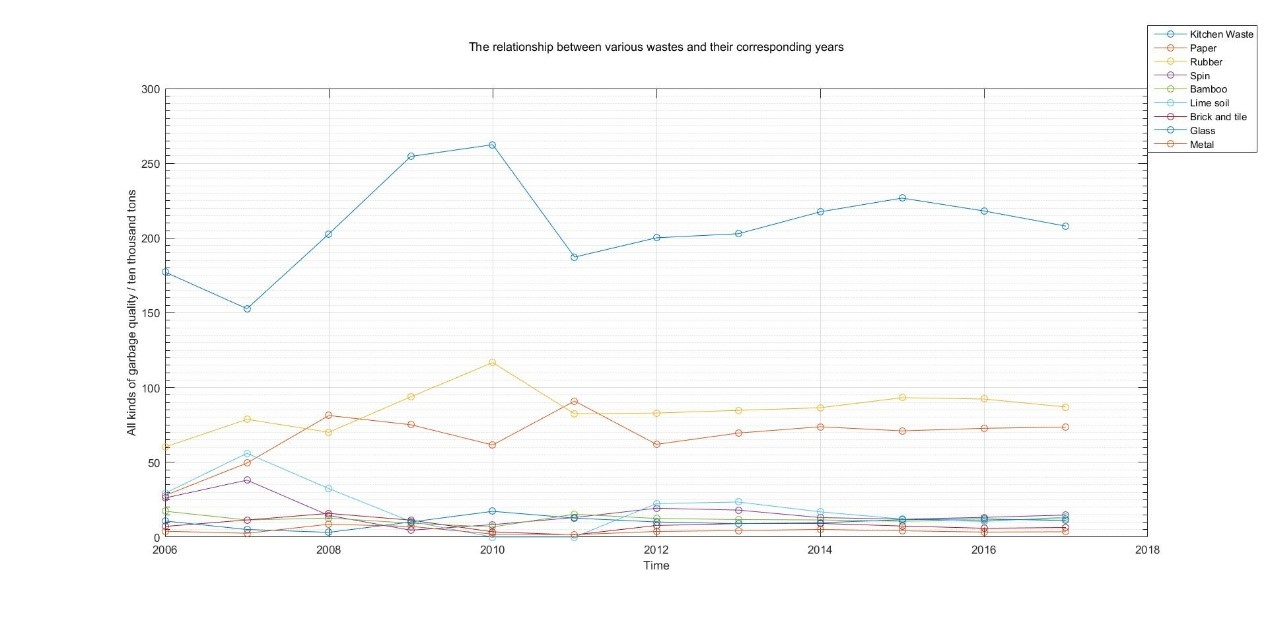
\includegraphics{Answer1.jpg}\\
\end{center}
\indent The results are showed visually on the above line chart.\\
\indent Finally, we got the amount of all kinds of garbage in Shenzhen, and after adding it up, we found that the total amount of garbage was smaller than the total amount of garbage from 2012 to 2016. So we can believe that our estimate of the amount of garbage in 2017 is accurate.\\
\begin{table}[h]
\caption{}
\begin{center}
\begin{tabular}{ccccccc}
\hline
Year&2009&2012&2013&2014&2015&2016\\
\hline
Relative Error&0.0056&0.1931&0.2001&0.2292&0.2157&0.0829\\
\hline
\end{tabular}
\end{center}
\end{table}\\
\newpage

\section{Model II}
\indent To solve this problem, we take advantage of the linear programming model which is used in assignment problem.
\subsection{Collection of the Data}
\indent In view of the population concentration and economic development of the central business district of a region, we consider that the entire waste of a region is produced by the central business district, where there is no particularly visible central business district. Priority is given to the choice of high-volume commercial streets and pedestrian streets.\footnote{The data comes from \textit{Baidumap}.}\\
\begin{table}[h]
\caption{}
\begin{center}
\begin{tabular}{cc}
\hline
Administrative region&The name of the prosperous area\\
\hline
Futian&Huaqiang North Commercial Street(Huaqiang North Road)\\
\hline
Luohu&South Commercial Plaza(Yongxin Road)\\
\hline
Yantian&Government of Yantian District\\
\hline
Nanshan&South Village Commercial Street\\
\hline
Baoan&Commercial Street\\
\hline
Longgang&Xintian commercial street\\
\hline
\end{tabular}
\end{center}
\end{table}\\
\indent The following table shows the shortest road distance between the central business district of Shenzhen and the waste treatment plant (considering that the garbage is transported by road).\footnote{The data comes from \textit{Baidumap}.}\\
\begin{table}[h]
\caption{Unit:km}
\begin{center}
\begin{tabular}{p{4cm}p{2cm}p{2cm}p{2cm}p{2cm}p{2cm}p{2cm}}
\hline
\indent Degrading treatment point of kitchen waste in Nanshan&Yantian Incineration Plant&Xiaping Landfill Site&Tiger pit environment garden&Pinghu Incineration Plant&Duck lake landfill\\
\hline
Futian&19.1&33.9&7.1&58.6&25.9&22.9\\
\hline
Luohu&21.2&23.7&13.8&60.6&21.3&16.8\\
\hline
Yantian&34.1&10.2&20.9&63.6&25.2&16\\
\hline
Nanshan&2.3&44.3&26.9&43.3&39.8&37.4\\
\hline
Baoan(including Guangming)&26.3&42.2&23&32.6&24.3&25.8\\
\hline
Longgang(including Pingshan)&26&29.5&14.4&61.6&17.6&17.2\\
\hline
\end{tabular}
\end{center}
\end{table}\\
\indent PS: There are both landfills and incinerators in the Tiger Pit Environment Park, which will be regarded as two overlapping treatment points to calculate the amount of MSW incineration and landfill separately.\\
\indent The following is the design processing capacity of the garbage disposal points in all areas of Shenzhen:\footnote{The data comes from reference 4 and 5.}\\
\begin{table}[h]
\caption{Unit:t/day}
\begin{center}
\begin{tabular}{cc}
\hline
Treatment plant&Processing capacity\\
\hline
Nanshan Waste Incineration Power Plant&800\\
\hline
Yantian Waste Incineration Power Plant&450\\
\hline
Tiger pit Waste Incineration Power Plant&4200\\
\hline
Pinghu Waste Incineration Power Plant&1675\\
\hline
Xiaping Solid Waste Landfill&3500\\
\hline
Tiger pit Solid Waste Landfill&1500\\
\hline
Longgang Pingxi Solid Waste Landfill&400\\
\hline
\end{tabular}
\end{center}
\end{table}\\
\indent The freight per ton of garbage per kilometre assumes a piece wise function relationship with the increase of transportation distance.\footnote{The data comes from reference 6.}
\[p(d)=\begin{Bmatrix}
60&0\leq d\leq 10\\
d+50&10\leq d\leq 20\\
1.5x+40&d\geq20
\end{matrix}
\right.\]
\[c_{ij}=p(d_{ij})d_{ij}\]
It is convenient to solve the equation if unification is regarded as 60 yuan per ton per kilometre.
\[p(d)=60\]
\[c_{ij}=60d_{ij}\]
\indent The government subsidy of 1 tons of landfill is about 60 yuan.\footnote{The data comes from reference 6.}\\
\indent The government subsidy of 1 tons of incineration is about 55 yuan.\footnote{The data comes from reference 7.}\\
\indent The waste gas generated from burning a garbage is \(23000\textrm{Nm}^3\). The exhaust gas temperature is estimated to be 150 degrees Celsius. The \textit{Clapeyron}'s ideal gas equation of state is used to convert the target to cubic meter, and then multiplied by air density 1294.64g/cm3. After unified unit, it has polluted about 18.45 tons of air.
\[23000\div2.5\times(273.15+150)\div273.15\times1294.64\div1000\div1000=18.45142825\]
\indent The harmful filtrate produced by a landfill of a landfill is 77.2 kilograms, and the dilution concentration is 1\%. The conversion unit pollutes about 7.72 tons of groundwater.
\[77.2\div1000\div0.01=7.72\]
\indent In 2016, a total of 323.82 tons of garbage and 248.46 tons of garbage were burned in Shenzhen. The total pollution caused by the upper formula was tons air and water. \footnote{The data comes from reference 3}
\[323.82\times10000\times18.45142825+248.46\times10000\times7.72=78931000\]
\indent In 2016, 62639 people in Shenzhen suffered from cancer, and the average cost of treatment for each cancer patient was 17088.01 yuan. Environmental pollution is one of the main causes of cancer hospitalization. The contribution of pollution to cancer hospitalization is regarded as 100\%, and the total cost of hospitalization is used as the total cost of pollution. \footnote{The data comes from reference 8.}
\[62639\times17088.01=107000000\]
\indent As a result, we can calculate the health costs of 1 and 2 per ton of waste and one ton of landfill waste, respectively.  \\
\[18.45142825\times\frac{107000000}{78931000}=250.2196\]
\[7.72 \times\frac{107000000}{78931000}=104.6908\]
\indent The proportion of various wastes estimated by first questions in 2017.\\
%%%
\indent Total social cost waste treatment in Shenzhen city is given in the data, the implementation of Shenzhen city garbage classification subsidy is 423 yuan per ton.\footnote{The data comes from reference 6.}\\
\indent Unrecyclable category accounted for about 60\% of the garbage after garbage disposal, proceed according to the above scheme, the remaining 40\% Recyclable garbage were assumed to be used completely, and not processed the cost of manufacturing, in the ideal case the product can be sold, Recyclable using garbage mainly include the following categories (because the metal cans, glass bottles and other products in the recovery of interest into the trash to be transported to the garbage recycling station will be picked up before the junkmen, so not much, the remaining available so negligible)\\
\begin{table}[h]
\caption{Unit:yuan/kg}
\begin{center}
\begin{tabular}{ccp{8cm}}
\hline
The use of unit&Income&Usages\\
\hline
Paper&0.4&Reengineering paper,paper recovery price\\
\hline
Plastic&1.5&Recycled plastic, plastic recovery price\\
\hline
Kitchen waste&1.2&Formation of biogas power generation by meal\\
\hline
Wood&6.667&M
akes plywood and so on. The average value of 35 Jin of plywood is 120 yuan.\\
\hline
\end{tabular}
\end{center}
\end{table}\\
\subsection{Foundation of the Model}
\indent We regard min P as objective function and list the formula:\\
\[\textrm{min }P=P_1+P_2+P_3\]
\indent The following is the linear constraint condition:
\[\textrm{s.t.}
\left\{
\begin{array}{lr}
\sum\limits_{j=1}^{7}x_{ij}=a_i\\
\sum\limits_{i=1}^{6}x_{ij}\leq b_j\\
x_{ij}\geq0\\
P_1=\sum\limits_{i=1}^6\sum\limits_{j=1}^7c_{ij}x_{ij}\\
P_2=\sum\limits_{j=5}^{7}60x_{ij}+\sum\limits_{j=1}^{4}55x_{ij}\\
P_3=\sum\limits_{j=5}^{7}104.6908x_{ij}+\sum\limits_{j=1}^{7}250.2196x_{ij}\\
\end{array}
\right.\]
\indent The solution which is eligible is called "feasible solution". The optimal solution is the solution that minimizes the value of the objective function.\\
\indent The total amount of waste in the second scheme is recalculated, and the total cost formula for recycling subsidies and recovery benefits is as follows:
\[P\prime=P|_{a_i=0.6a_i}+432\times\sum\limits_{i=1}^6a_i-0.4\times\sum\limits_{i=1}^6a_i\times\sum\limits_{j=1}^4q_jm_j\]
\subsection{Model Results}
\indent The optimal transport scheme for scheme 1 is as follows (less than 0.001 in place of 0) (unit: tons):\\
\begin{table}
\caption{Unit:t}
\begin{center}
\begin{tabular}{p{4cm}p{2cm}p{2cm}p{2cm}p{2cm}p{2cm}p{2cm}}
\hline
&Nanshan kitchen waste degradation treatment point & Yantian incineration plant & Xia Ping landfill site&tiger pit environmental Park & Pinghu incineration plant &Yahu landfill \\
\hline
Futian&0.00 &0.00 &0.00 &556676.09 &0.00 &0.00\\
\hline
Luohu&0.00 &0.00 &0.00 &173431.07 &0.00 &146000.00\\
\hline
Yantian&0.00 &90720.17 &0.00 &0.00 &0.00 &0.00\\
\hline
Nanshan&292000.00 &0.00 &0.00 &163534.58 &0.00 &0.00\\
\hline
Baoan(including Guangming)&0.00 &0.00 &31278.00 &0.00 &458642.62 &0.00\\
\hline
Longgang(including Pinghu)&0.00 &0.00 &580097.00 &383858.27 &0.00 &0.00\\
\hline
\end{tabular}
\end{center}
\end{table}\\
\indent The optimal transport scheme of scheme two is the same as that of the scheme one.\\
\indent The pollution and disposal of the waste and the cost of the 2 schemes are as follows :\\
\begin{table}
\caption{Unit:t}
\begin{center}
\begin{tabular}{ccc}
\hline
Scheme&The mass of rubbish incinerated&The mass of rubbish landfilled\\
\hline
1&2344458.25&1882142.62\\
\hline
2&1406674.95&1129285.57\\
\hline
\end{tabular}
\end{center}
\end{table}\\
\begin{table}
\caption{Unit:t}
\begin{center}
\begin{tabular}{ccc}
\hline
Scheme&The mass of air polluted&The mass of water polluted\\
\hline
1&43255255&14530141\\
\hline
2&25953153&8718084.6\\
\hline
\end{tabular}
\end{center}
\end{table}\\
\begin{table}[h]
\caption{Unit:yuan}
\begin{center}
\begin{tabular}{cccccc}
\hline
Scheme&Total cost&Transportation cost&Treatment cost&Health cost&Recycling cost\\
\hline
1&6752819140.942&5520488357.622&61209416.98&1171121366.3367&0\\
\hline
2&4294802287.89&3312293014.573&36725650.189&702672819.80&243110803.32\\
\hline
\end{tabular}
\end{center}
\end{table}\\
\newpage

\section{Model III}
\indent In this part, we introduce principal component regression analysis into the question. This analytical method was created to overcome instability of least square estimation when the data matrix exists multicollinearity. The principal component means changing the regression argument to a set of variables. We choose a part of important principal component as new variables and give up the variable which has weak effects on the problem in order to reduce dimension. Then, we harness the least square method to estimate the model parameter and turn to the original model to estimate the parameter.
\subsection{Collection and Operation of the Data}
\indent The following is a city in 2016 that sold the amount of waste per meal.\footnote{The data comes from \textit{iResearch}' s analysis of the big data on \textit{Are You Hungry}.}\\
\begin{table}[h]
\caption{}
\begin{center}
\begin{tabular}{ccc}
\hline
Ranking &City&Ratio\\
\hline
1&Chengdu&1.187\\
\hline
2&Xi’an&1.185\\
\hline
3&Hangzhou&1.178\\
\hline
4&Suzhou&1.165\\
\hline
5&Nanjing&1.137\\
\hline
6&Shanghai&1.133\\
\hline
7&Beijing&1.119\\
\hline
8&Qingdao&1.106\\
\hline
9&Fuzhou&1.094\\
\hline
10&Wenzhou&1.072\\
\hline
&National average&1\\
\hline
\end{tabular}
\end{center}
\end{table}\\
\indent PS: The national average 3.27 boxes outside takeaway calculation.\\
\indent We selected 2 mega cities: Beijing, Shanghai and 4 first tier cities: Chengdu, Xi'an, Hangzhou and Nanjing, mainly because these cities are representative and have complete data.\\
\indent The following is the monthly average order volume in the six cities in 2016.\footnote{The data comes from \textit{Amoy Stock}' s analysis of the big data on \textit{Baidutakeaway}.}\\
\begin{table}[h]
\caption{Unit:10000 orders}
\begin{center}
\begin{tabular}{ccccccc}
\hline
Cities&Chengdu&Xi'an&Hangzhou&Nanjing&Shanghai&Beijing\\
\hline
\(n_{\textrm{m}}\)&19&28&22&29&75&343\\
\hline
\end{tabular}
\end{center}
\end{table}\\
The following is the total population of the 6 major cities:\footnote{The data comes from the National Bureau of Statistics.}\\
\begin{table}[h]
\caption{10000 people
}
\begin{center}
\begin{tabular}{ccccccc}
\hline
Cities&Chengdu&Xi’an&Hangzhou&Nanjing&Shanghai&Beijing\\
\hline
\(n_{\textrm{p}}\)&1591.8&879.56&918.8&827&2419.7&2170.5\\
\hline
\end{tabular}
\end{center}
\end{table}\\
\indent In 2016, the formula for calculating the quantity of food boxes outside the city was:
\[12n_{\textrm{m}}\times3.27r\div n_{\textrm{p}}=y\]
\indent Considering the possible factors related to take-out garbage manufacturing, we chose overtime rate \(x_1\)\footnote{The data comes from  \textit{Kelly} survey company.}, average stay up time \(x_2\)\footnote{The data comes from \textit{Huami Technology} collected the national \textit{Xiaomi} ring users.}, average income \(x_3\)\footnote{The data comes from China's Bureau of Statistics.}, consumption level \(x_4\) 4 indicators. And the average income and consumer price index for less than eight hours of stay up (in minutes).Considering that the consumer price index was calculated at 100 in the previous year. That is, it is also related to the data of the year before. So take the average CPI\footnote{The data comes from China's Bureau of Statistics.} for 2015 and 2016 as an indicator of consumption level.
\begin{table}[h]
\centering
\caption{}
\begin{tabular}{ccccccc}
\hline
Cities& Chengdu & Xi'an & Hangzhou & Nanjing & Shanghai & Beijing \\
\hline
\(t_{\textrm{sleep}}\)& 0:06    & 23:56 & 23:45    & 23:43   & 23:42    & 23:41\\
\hline
\(t_{\textrm{wake\ up}}\) & 7:52    & 7:40  & 7:32     & 7:28    & 7:33     & 7:33 \\
\hline
\end{tabular}
\end{table}\\
\[x_2=60(8-(t_{sleep}-t_{wake\ up}))\]
\begin{table}[h]
\centering
\caption{}
\begin{tabular}{ccccccc}
\hline
Cities        & Chengdu & Xi'an  & Hangzhou & Nanjing & Shanghai & Beijing \\
\hline
CPI_{2015} & 101.10  & 101.80 & 101.70   & 101.10  & 102.40   & 101.80  \\
\hline
CPI_{2016} & 102.20  & 100.90 & 102.70   & 102.70  & 103.30   & 102.10\\
\hline
\end{tabular}
\end{table}\\
\[x_4=\frac{(\textrm{CPI}_{2015}+\textrm{CPI}_{2016})}{2}\]
\subsection{Foundation of the Model}
\indent We select six cities, including Beijing, Shanghai, Nanjing, Xi’an, Chengdu, Hangzhou to study the relationship between the number of waste produced by takeaways and the characteristic of residents. As for the characteristics, we just choose four index, which is the overtime rate, average time of staying up late, average revenue and consumer price index.\\
\indent The following table is some data about the relationship between takeaways’ waste and the four indexes that we collect.\\
\begin{table}[h]
\caption{}
\begin{center}
\begin{tabular}{cccccc}
\hline
Cities&\(x_1\)&\(x_2\)&\(x_3\)&\(x_4\)&\(y\)\\
\hline
Beijing&0.91894484&0.54&14&6941&101.65\\
\hline
Shanghai&2.472016113&0.65&16&7556&101.35\\
\hline
Nanjing&1.829450271&0.72&13&7608&102.2\\
\hline
Xi'an&2.585988428&0.59&15&7342&101.9\\
\hline
Chengdu&2.277735407&0.52&9&9802&102.85\\
\hline
Hangzhou&11.46932978&0.54&8&9942&101.95\\
\hline
\end{tabular}
\end{center}
\end{table}\\
\indent When we set these variables, what we should do is to derive the empirical regression equation:
\[\hat{y}=k_0+k_1x_1+k_2x_2+k_3x_3+k_4x_4\]
\subsection{Model results}
\indent With the help of MATLAB, we can derive the correlation coefficient matrix,all the eigenvalues and the contribution ratas:
\[R=\begin{bmatrix}
1.0000&0.5259&-0.4906&-0.2609\\
0.5259&1.0000&-0.9291&-0.6787\\
-0.4906&-0.9291&1.0000&0.6209\\
-0.2609&-0.6787&0.6209&1.0000
\end{bmatrix}\]
\[V=\begin{bmatrix}
-0.3847& 0.8389 &-0.3815&-0.0511\\
 -0.5723&-0.0674& 0.3286&0.7483\\
0.5576&  0.0654&-0.5063&0.6546\\
0.4621& 0.5361&0.7001&0.0943
\end{matrix}\]
\[\Lambda=\begin{bmatrix}
2.8068\\
0.7528\\
0.3747\\
0.0658
\end{bmatrix}\]
\[C=\begin{bmatrix}
0.7017\\
0.8899\\
0.9836\\
1.0000
\end{bmatrix}\]
\indent On top of the vectors, we calculate all principal component scores and obtain the matrix:
\[S=\begin{bmatrix}
-0.8309&-1.0157&0.4404&-0.3076\\
-1.7340&-0.1548&-0.5428&0.3280\\
-0.7679&1.5509&-0.0480&-0.2223\\
-0.8582&-0.2169&0.4828&0.1334\\
2.4329&0.2666&0.5734&0.2030\\
1.7583&-0.4300&-0.9059&-0.1347
\end{bmatrix}\]
\indent By calculating the cumulative, we decide to discard the two latter characteristic values since their contribution could be ignored. The Eigenvectors corresponding to the two former eigenvalues are:
\[v_1=\begin{bmatrix}
-0.3847\\
 -0.5723\\
0.5576\\
0.4621
\end{bmatrix}\]
\[v_2=\begin{bmatrix}
0.8389\\
-0.0674\\
0.0654\\
0.5361
\end{bmatrix}\]
\indent We can see that the first eigenvector and overtime rate, night time is inversely proportional, proportional to the income level and consumption level, which may be called the quality of life of principal component \(z_1\), and the second feature vector and overtime rate, proportional to the apparent consumption level, may be called economic level of principal component \(z_2\), so we have:\\
\[\hat{y}=0.3107z_1-0.2288z_2\]
\indent In the end, we operate principal component regression analysis to obtain the regression equation. When we restore it to the original independent variable, we derive the final result:
\[\hat{y}=-4.787862-15.623363x_1-0.193927x_2+0.000469x_3+0.159129x_4\]
\indent The residual standard deviation is calculated as 3.6269.
\newpage

\section{Short essay}
\begin{center}
\bf\large A report on the study of takeaway waste
\end{center}
\indent Solid waste has become one of the main pollution to the environment. But some time ago on the Internet takeaway garbage blamed on the crest of a wave takeaway, sparked a debate. In view of the problem of solid garbage disposal and the overstatement of the accusation of foreign selling, this paper uses data to carry out quantitative analysis. \\
\indent First of all, this paper selects Shenzhen as the research site. According to the historical sampling survey data of the garbage components in different\\
\indent  districts, we use the weighted average of the population of each district to get the garbage components of Shenzhen, and calculate the quality of all kinds of garbage in Shenzhen with the total amount of garbage in Shenzhen. After obtaining the time series of all kinds of garbage quality in Shenzhen, we estimated the garbage quality after a few years with an exponential smoothing method. The relative error between the obtained data and the existing data is about 1\%. We believe that the estimate for 2017 is accurate.\\
\indent Then, using the data of the first question, this paper begins to solve the optimal solution of the garbage disposal. It is divided into 2 cases that do not carry out the classification of garbage and carry out the classification of garbage. Considering the transportation cost and processing cost of garbage, this paper considers the importance of environmental protection, calculates the cost of health by using the cost of cancer hospitalization, and sets the minimum cost plan as the best plan. On the one hand, the government has to pay extra garbage sorting subsidies, but relatively, the garbage that is not recyclable and has to be processed will also be reduced, and the remaining recyclable garbage can generate new economic benefits through reusing. After comparison, it is concluded that the reasonable scheduling of garbage classification and garbage transportation can greatly reduce the total cost, that is, the optimal scheme.\\
\indent After obtaining the relevant data of solid waste, this paper began to study the related factors of the production of the refuse. Considering the 4 indicators, such as overtime rate, late night time, residents' income and consumption level, we use principal component regression to analyze the relationship between takeaway garbage and residents' living habits. In the first 2 principal components were obtained through a significant test of the variance of the experience of a linear regression, 2 principal components can be regarded as the quality of life and economic level of principal component principal component explains 2 reasons for takeout waste, on the other hand, using the experience of linear regression estimation take away other City garbage.\\
\indent By comparing the estimated result of third problem and the data obtained can be found in a big city like Shenzhen economic development, per capita annual production of only 3 to 4 take away waste plastic lunch box, while the per capita per year compared to manufacturing plastic waste is 50 kg or more, can be seen on the plastic waste is not big takeaway. Of course, the non-repudiation of takeout also plays a role that cannot be ignored.\\
\indent To sum up, we should take a reasonable look at the impact of takeout on the environment, but caring about environmental protection is not a bad thing, at the same time, it also improves people's attention to environmental protection. It can be seen that the concept of environmental protection has been deeply rooted in the hearts of the people.
\newpage

\section{Strength and Weakness}
\subsection{Strength}
The first time series model can forecast the number of different types of solid waste to the far future more precisely, thus reminding the whole society to do actions.
The second model propose a more practical and optimized scheme to do garbage disposal. We convert the quantitative analysis into the treatment cost. From the perspective of economy, the more optimized solution is recycling and such a cost-effective result should be generalized among citizens.
The third model objectively study the relationship between the waste caused by takeaways and the characteristic of residents in a quantitative way through the establishment of index system.
We neglect some irrelevant factors when analyzing corresponding problem. We use a simplified model to reflect the actual situation objectively.
\subsection{Weakness}
For the first model, we need to collected a large number of data to estimate the number in the future, which is fussy to realize.
For the second model,
For the third model, the index that we select is incomplete and there are also so many factors having effect on the results.
\newpage

\section{Reference}
\begin{enumerate}[(1)]
\item Basic Data on Environmental Garbage in Shenzhen,Environmental health management department
\item Shenzhen Statistical Yearbook , Shenzhen statistical bureau
\item Statistical data on Urban Management,Shenzhen urban management
\item List of Municipal Solid Waste Landfill in Shenzhen (June 2016),Shenzhen urban management
\item List of Municipal Solid Waste Incineration Power Plants in Shenzhen (June 2016),Shenzhen urban management
\item A Study on the Total Social Cost of Municipal Solid Waste Disposal in Shenzhen,Chinese knowledge internet
\item Simple Cost Analysis of Waste Incineration Power Generation,Chinese knowledge internet
\item Summary of Health Statistics in Shenzhen,Health and family planning commission
\item Shoukui Si, Xijing Sun: Mathematical Modeling, 2011
\end{enumerate}
\newpage

\section{Appendix}
Here are some simulation programmers we used in our models:
\subsection{Model I}\footnote{The code of reference 9 is used for reference.}
\begin{lstlisting}[title=problem1.m, frame=shadowbox]
function [change]=pq(y,o)
for q=1:6
    if q>1

    e=y_yhat2017';

    for w=1:5

        y(w,:)=y(w+1,:);
    end
    y(w+1,:)=e(n+1,:);
    end

yt=y;
n=length(yt(:,1));
alpha=[0.3 0.5 0.8];m=length(alpha);
for i=1:o
yhat(1,1:m,i)=(yt(1,i)+yt(2,i))/2;
end

for i=1:o
    for j=2:n
    yhat(j,:,i)=alpha*yt(j-1,i)+(1-alpha).*yhat(j-1,:,i);

    end
end
yhat;
for i=1:o
yhat2017(i,:)=alpha*yt(n,i)+(1-alpha).*yhat(n,:,i);
end
for i=1:o
y_yhat2017(i,:)=[y(:,i)' yhat2017(i,2)];
end
r=y_yhat2017';
if q>1
    change(n+q,:)=r(n+1,:);
else
    change=r;
end
end
function createfigure(X1, YMatrix1)
%CREATEFIGURE(X1, YMATRIX1)
%  X1: The vector of X data
%  YMATRIX1:  Y data matrix
% found figure
figure1 = figure;
% found axes
axes1 = axes('Parent',figure1,...
    'Position',[0.13 0.132714369680176 0.775 0.72418511924657]);
hold(axes1,'on');
% Creating multiple rows using plot's Matrix input
plot1 = plot(X1,YMatrix1,'Marker','o','Parent',axes1);
set(plot1(1),'DisplayName','Kitchen Waste');
set(plot1(2),'DisplayName','Paper');
set(plot1(3),'DisplayName','Rubber');
set(plot1(4),'DisplayName','Spin');
set(plot1(5),'DisplayName','Bamboo');
set(plot1(6),'DisplayName','Lime soil');
set(plot1(7),'DisplayName','Brick and tile');
set(plot1(8),'DisplayName','Glass');
set(plot1(9),'DisplayName','Metal');
% found xlabel
xlabel({'Time',''});
% found ylabel
ylabel({'All kinds of garbage quality / ten thousand tons'});
% found title
title({'The relationship between various wastes and their corresponding years','',''});
box(axes1,'on');
% Setting the rest of the coordinate axis properties
set(axes1,'LineStyleOrderIndex',2,'XGrid','on','YGrid','on','YMinorGrid',...
    'on','YMinorTick','on');
% found legend
legend1 = legend(axes1,'show');
set(legend1,...
'Position',[0.846527777405249 0.644997106275451 0.0520833337058624 0.329358326447816]);
function [change]=pq(y,o)
for q=1:6
if q>1
    e=y_yhat2017';
    for w=1:5
    y(w,:)=y(w+1,:);
    end
    y(w+1,:)=e(n+1,:);
    end
yt=y;
n=length(yt(:,1));
alpha=[0.3 0.5 0.8];m=length(alpha);
for i=1:o
yhat(1,1:m,i)=(yt(1,i)+yt(2,i))/2;
end
for i=1:o
    for j=2:n
    yhat(j,:,i)=alpha*yt(j-1,i)+(1-alpha).*yhat(j-1,:,i);
    end
end
yhat;
for i=1:o
yhat2017(i,:)=alpha*yt(n,i)+(1-alpha).*yhat(n,:,i);
end
for i=1:o
y_yhat2017(i,:)=[y(:,i)' yhat2017(i,2)];
end
r=y_yhat2017';
if q>1
    change(n+q,:)=r(n+1,:);
else
    change=r;
end
end
\end{lstlisting}
\subsection{Model II}\footnote{The code of reference 9 is used for reference.}
\begin{lstlisting}[title=problem2.m, frame=shadowbox]
yn=[49.23 	7.73 	16.74 	7.27 	4.81 	8.15 	1.98 	2.99 	1.09
37.53 	12.17 	19.35 	9.36 	2.81 	13.77 	2.81 	1.25 	0.63
45.98 	18.44 	15.90 	3.28 	2.89 	7.35 	3.59 	0.72 	1.95
54.79 	12.86 	24.37 	1.74 	1.41 	0.00 	0.73 	3.60 	0.42
40.89 	19.86 	18.00 	2.86 	3.34 	0.00 	0.33 	2.77 	0.36 ];
x=[2006 2007 2008 2010 2011];
yn=[yn(1,:)*360 ; yn(2,:)*407; yn(3,:)*441;yn(4,:)*479; yn(5,:)*458];
yn=yn/100;
ym=yn';
for i=1:9
    jie(i)=interp1(x,ym(i,:),2009,'spline');
end
jie
y=[yn(1,:);yn(2,:);yn(3,:);jie;yn(4,:);yn(5,:)];
q=[
120.24	123.36	126.56	129.85	131.96	132.52
87.29	88.55	89.83	91.13	92.45	93.1
21.44	21.31	21.17	21.04	20.91	21.1
94.55	98.22	102.03	105.99	108.94	109.99
353.24	376.93	400.9	424.37	450.51	454.84
194.34	204.01	213.78	222.63	232.43	235.19
];
w=pq(q',6);
qs=pq(y,9);
itrash=[sum(qs(4,:)) sum(qs(7,:)) sum(qs(8,:)) sum(qs(9,:)) sum(qs(10,:)) sum(qs(11,:))]
rtrash=[479.25 521.69	541.14	574.81	572.28	479.25]
wucha=abs((rtrash-itrash)./rtrash);
x=2006:1:2017;
createfigure(x, qs);
qsa=qs(12,:)*10000;
qss= sum(qs(12,:))*10000;
wi=w(12,:);
wip=wi/sum(wi);
a=qss*wip;
bt=[3500 1500 400];
bt=bt*365;
bf=[800 450 1675 4200];
bf=bf*365;
d=[
    19.1	33.9	25.9	58.6	7.1	58.6	22.9 21.2	23.7	21.3	60.6	13.8	60.6	16.8 34.1	10.2	25.2	63.6	20.9	63.6	16 2.3	44.3	39.8	43.3	26.9	43.3	37.4 26.3	42.2	24.3	32.6	23	32.6	25.8 26	29.5	17.6	61.6	14.4	61.6	17.2
];
x=ones(1,42);
p2=x;
p=60;
c=p*d;
p1=c;
for i=1:6
    p2(5*i)=60;
    p2(6*i)=60;
    p2(7*i)=60;
    p2(1*i)=-432;
    p2(2*i)=-432;
    p2(3*i)=-432;
    p2(4*i)=-432;
end
\end{lstlisting}
\subsection{Model III}\footnote{The code of reference 9 is used for reference.}
\begin{lstlisting}[title=problem3.m, frame=shadowbox]
clc,clear
load data3.txt
[m,n]=size(data3);
x=data3(:,[2:n])
y=data3(:,1)
h1=[ones(m,1),x]\y;
h1=h1';
r=corrcoef(x)
xd=zscore(x)
yd=zscore(y)
[vec1,lamda,rata]=pcacov(r)
f=repmat(sign(sum(vec1)),size(vec1,1),1);
vec2=vec1.*f
contr=cumsum(rata)/sum(rata)
df=xd*vec2
num=input('Please input the number of principal components:')
h21=df(:,[1:num])\yd
h22=vec2(:,1:num)*h21
h23=[mean(y)-std(y)*mean(x)./std(x)*h22,std(y)*h22'./std(x)]
fprintf('y=%f',h23(1));
for i=2:n
    if h23(i)>0
        fprintf('+%f*x%d',h23(i),i-1);
    else
        fprintf('%f*x%d',h23(i),i-1);
    end
end
fprintf('\n')
rmse=sqrt(sum((h23(1)+x*h23(2:end)'-y).^2)/(m-num))

\end{lstlisting}
\end{document}

